\chapter{Dagens pasientsignalsystem ved St. Olavs Hospital}
\label{appendix_dagenssystem}

St. Olavs Hospital er et universitetssykehus eid av Helse Midt-Norge RHF. I 2012 hadde sykehuset 131 547 inneliggende pasienter, 1 008 senger og 9 584 ansatte totalt. 
I dette appendikset vil vi beskrive dagens pasientsignalsystem, basert på informasjon gitt av Brukermanual for Pasientsignal og Pasientsignalapplikasjon (ref kilde).

\section{Pasientsignal}
Et pasientsignal utløses i et rom ved et sengetun for å tilkalle/alarmere pleiepersonell.
Vi vil skille mellom to typer signaler, tilkalling og hasteanrop, hvor tilkalling utløses av pasient, mens hasteanrop utløses av pleiepersonell. 
Dagens system er sammensatt av et fast system og et trådløst system. Det faste systemet, også refererert til som pasientsignalanlegget, består av fastmonterte paneler med trekksnorer og/eller trykknapper: anropspanel \ref{anropspanel}, rompanel \ref{rompanel} og vaktromsapparat \ref{vaktromsapparat}.

\begin{figure}[H]
        \centering
        \begin{subfigure}[b]{0.3\textwidth}
        		\centering
                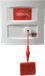
\includegraphics[scale=0.7]{anropspanel.png}
                \caption{Anropspanel}
                \label{anropspanel}
        \end{subfigure}%
        \begin{subfigure}[b]{0.3\textwidth}
        		\centering
                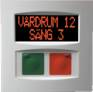
\includegraphics[scale=1.5]{rompanel.jpg}
                \caption{Rompanel}
                \label{rompanel}
        \end{subfigure}
        \begin{subfigure}[b]{0.3\textwidth}
        		\centering
                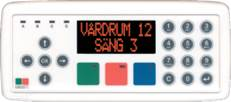
\includegraphics[scale=1]{vaktromsapparat.jpg}
                \caption{Vaktromsapparat}
                \label{vaktromsapparat}
        \end{subfigure}
        \caption{Pasientsignalanlegget}\label{pasientsignalanlegget}
\end{figure}
\noindent
Det finnes to typer anropspanel, et for våtrom og et for vanlig rom. I vanlige rom er anropspanelet plassert ved sengen, og har en trykknapp med lysdiode og en trekksnor.
Trykknappen utløser et hasteanrop, mens trekksnoren utløser en tilkalling.

\noindent
Rompanelet er plassert ved døren til hvert av rommene på et sengetun. Det har et display, og en grønn og en rød trykknapp med hver sin lysdiode. Grønn knapp trykkes for å markere tilstedeværelse eller for å avslutte et hasteanrop. Rød knapp trykkes for å utløse en tilkalling, eller et hasteanrop etter at tilstedemarkering er aktivisert. Rød knapp kan også holdes inne i 2 sekunder for å utløse hasteanrop, dersom tilstedemarkering ikke er aktivert. 

\noindent
Vaktromsapparatet er sentralt plassert i det åpne landskapet på sengetunet. Det består av et display og flere tall- og tegntaster. Displayet indikerer stedangivelse for en tilkalling, hasteanrop og tilstedemarkerte rom. Tilkallinger og hasteanrop er signalisert med rød tekst, mens tilstedemarkering er vist ved grønn tekst. Tastene brukes for å programmere apparatet.

\noindent
Disse er videre tilkoblet det trådløse systemet, som består av følgende IKT-komponenter: pasientsignalapplikasjon \ref{pasientapplikasjon}, telefon \ref{telefon} og pasientterminal \ref{pasientterminal}.

\begin{figure}[H]
        \centering
        \begin{subfigure}[b]{0.35\textwidth}
        		\centering
                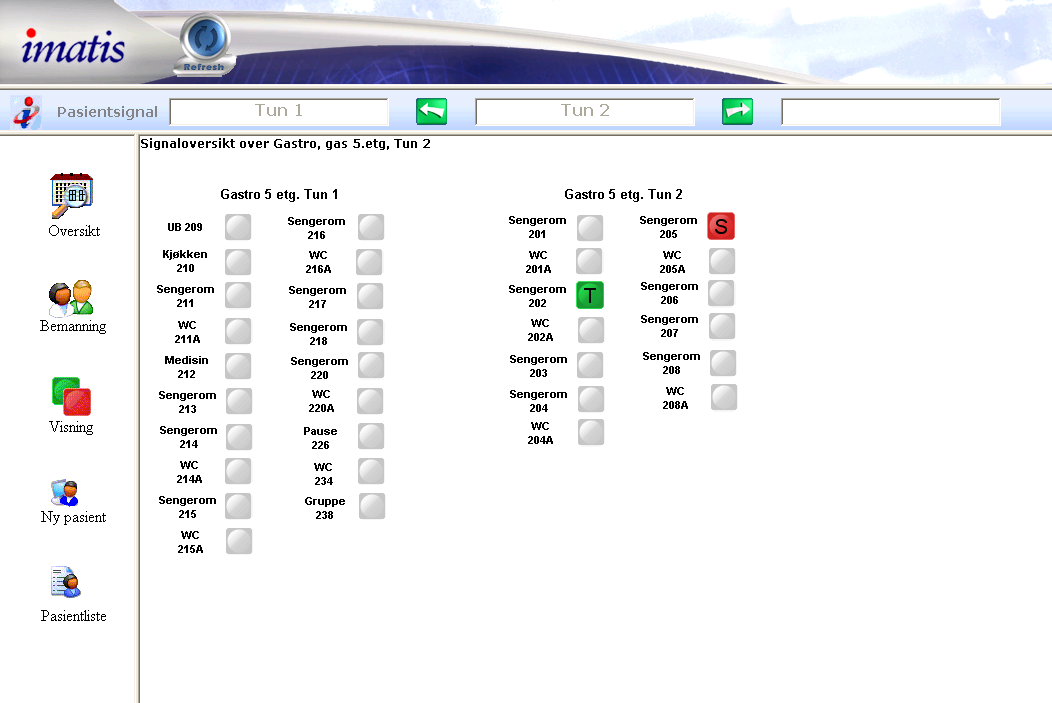
\includegraphics[scale=0.4]{pasientapplikasjon.png}
                \caption{Pasientsignalapplikasjon}
                \label{pasientapplikasjon}
        \end{subfigure}%
        \begin{subfigure}[b]{0.25\textwidth}
        		\centering
                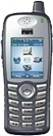
\includegraphics[scale=1]{telefon.jpg}
                \caption{Telefon}
                \label{telefon}
        \end{subfigure}
        \begin{subfigure}[b]{0.3\textwidth}
        		\centering
                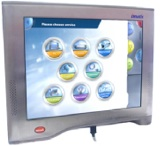
\includegraphics[scale=0.4]{pasientterminal.jpg}
                \caption{Pasientterminal}
                \label{pasientterminal}
        \end{subfigure}
        \caption{Det trådløse systemet}\label{dettradlosesystemet}
\end{figure}
\noindent
Pasientsignalapplikasjonen kjører på hvert sengetuns PC, 24 timer i døgnet, hver dag. Applikasjonen tilbyr i hovedsak fem funksjoner: (1) oversikt, (2) bemanning, (3) visning, (4) ny pasient og (5) pasientliste. Vi vil her utdype funksjonene bemanning og visning, da disse er av mest relevans for vår oppgave.  

\noindent
Bemanningsplanen, vist i figur \ref{bemanningsplan}, knytter tilgjengelig pleiepersonell til rommene ved et sengetun. Tilkallinger vil dermed sendes til riktig mottaker på bakgrunn av bemanningsplanen. 
\begin{figure}[H]
\centering
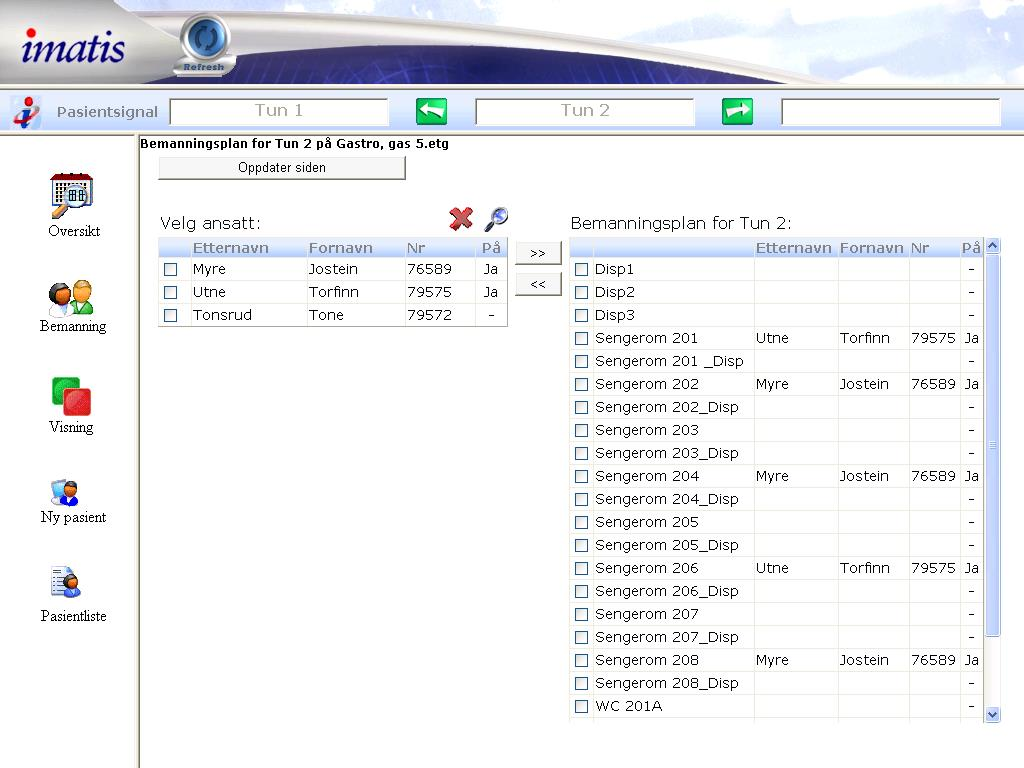
\includegraphics[scale=0.4]{bemanningsplan.jpg}
\caption{Bemanningsplan}
\label{bemanningsplan}
\end{figure}
\noindent
Funksjonen visning, vist i figur \ref{visning}, viser en oversikt over pasientsignalanlegget ved det gjeldende sengetunet.
\begin{figure}[H]
\centering
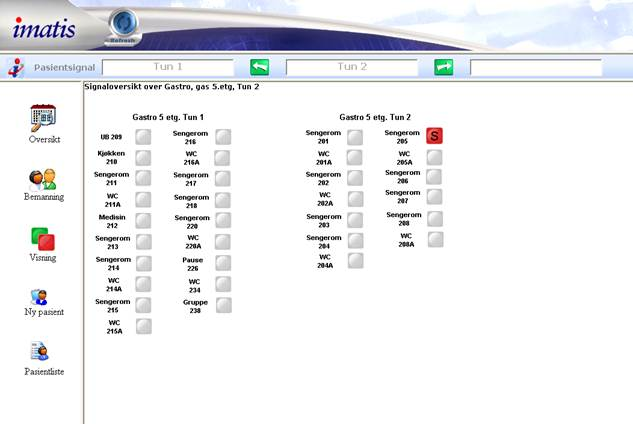
\includegraphics[scale=1]{normalvisning.jpg}
\caption{Visning}
\label{visning}
\end{figure}















